%Please insert your deliverables for Stage4 as follows:

We developed a User Interface using the package \textit{Tkinter}.  \textit{Tkinter} is a standard Python interface to TK Gui toolkit, which allows us to generate an interface  to guide users through our recommendation system.  Figures below are the demonstration of the UI.
\begin{itemize} 
\item{The initial statement to activate the application with the corresponding initial UI screenshot.}
\\Run the Python script named \textit{GUIpart} to start the UI. The initial nterface is shown below:
\begin{figure}[h] 
	\begin{center}
		\advance\rightskip-1cm
		{\scalebox{0.3}{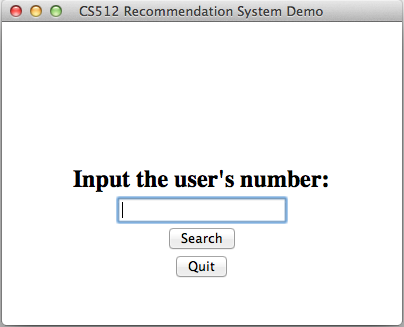
\includegraphics[width=300mm]{UI_Input.png}}}
		\caption{An example of finding the recommendations for user 1}\label{fig:UI_input}
	\end{center}
\end{figure}



\item{}
	The error messages popping-up when users access and/or updates are denied (along with explanations and examples):
	\begin{itemize} 
	\item{The error message: This is an invalid input, please input an integer between 0 to 32133. }
	\item{The error message explanation (upon which violation it takes place):  }
	The error pops up when the input number is out of range, i.e. the input user is not in the database. So the system cannot find such user.
	\item{The error message example according to user(s) scenario(s): Input user number 1000000.}
	\begin{figure}[h] 
	\begin{center}
		\advance\rightskip-1cm
		{\scalebox{0.3}{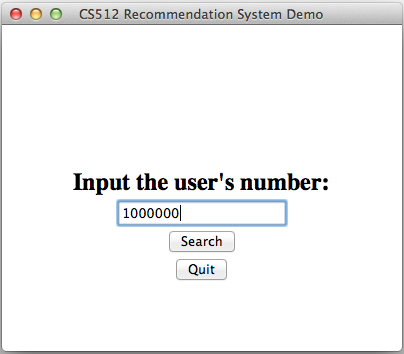
\includegraphics[width=300mm]{UI_Error1.png}}}
	\end{center}
	\end{figure}
	\begin{figure}[h] 
	\begin{center}
		\advance\rightskip-1cm
		{\scalebox{0.3}{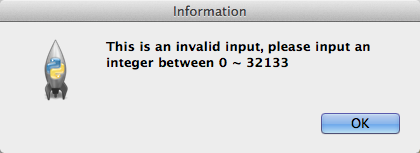
\includegraphics[width=300mm]{UI_Error2.png}}}
		\caption{Error message for inputting invalid user number 1000000}\label{fig:UI_Error}
	\end{center}
	\end{figure}
	
	 \end{itemize}
\item{}
	The information messages or results that pop-up in response to user interface events.
	\begin{itemize} 
	\item{The information message: shown in Fig. 11.}
	\begin{figure}[h] 
	\begin{center}
		\advance\rightskip-1cm
		{\scalebox{0.3}{\includegraphics[width=300mm]{UI_Result.png}}}
		\caption{UI demonstration of resulting recommendation for user 1}\label{fig:UI_Result}
	\end{center}
	\end{figure}
	\item{}
	The recommendation list contains 10 business units that are most likely favorable by input user. 
	 \end{itemize}


